\documentclass[a4paper,11pt]{article}
\usepackage[a4paper]{geometry}
\usepackage{polski}
\usepackage[polish]{babel}
\usepackage[utf8]{inputenc}

\usepackage{indentfirst} %taby na początku
\usepackage{graphicx} %dodawanie obrazków
\usepackage{subcaption}

\usepackage{lastpage} %znacznik ostatniej strony
\usepackage{fancyhdr} %odblokowanie wyglądu fancy
\usepackage{hyperref} %hiperłącza
\usepackage{float} %latające napisy
\usepackage{chngcntr} %zmiana countera

\usepackage{amsmath} %konieczne do matmy
\usepackage{amsfonts} %konieczne do czcionek mathbb
\usepackage{mathrsfs} %konieczne do czcionek mathscr
\usepackage{relsize}

\usepackage{tikz} %rysowanie obrazów
\usepackage{pgfplots}
\usepackage{siunitx}
\usepackage{rotating}
\usepackage{xcolor}

\usepackage{adjustbox}
\usepackage{multirow}
\usepackage{tabularx}
\usepackage{chngpage}
\usepackage{enumitem}
\usepackage{pdflscape}

\usepackage{listings}
\usepackage[paper=portrait,pagesize]{typearea}

\graphicspath{ {../Images/} }

\usetikzlibrary{arrows.meta,arrows}
\lstset{basicstyle=\small\ttfamily,breaklines=true,tabsize=2,numbers=left,showstringspaces=false,commentstyle=\color{red},keywordstyle=\color{blue}}
%head & foot
\counterwithin*{section}{part}
\pagestyle{fancy}
\title{Notatki}
\author{Mateusz Łuczak}
\date{}
\setlength\parindent{24pt}
\setlength{\headheight}{16pt}
\lhead{}
\rhead{}
\rfoot{str. \thepage/\pageref{LastPage}}
\cfoot{}
%do linii na górze
\renewcommand{\headrulewidth}{0pt}

\pgfplotsset{compat=newest}
\usepgfplotslibrary{units}

%\KOMAoptions{paper=landscape,pagesize}
%\recalctypearea
%end of preamble
\begin{document}

\thispagestyle{empty}
\begin{center}
	\textsc{\LARGE Politechnika Warszawska}\\[1.5cm]

	\textsc{\Large Wydział Elektryczny}\\[0.5cm]

	\textsc{\large Informatyka Stosowana}\\[2cm]

	\rule{\linewidth}{0.5mm}

	\textsc{\Large Dokumentacja projektowa}\\[0.5cm]

	\textit{Projektowanie graficznych interfejsów użytkownika} (1DI1732)

	\rule{\linewidth}{0.5mm}\\[3cm]

	\normalsize
	Krzysztof Dąbrowski (293101)

	Mateusz Łuczak (291088)
\end{center}

\newpage
\tableofcontents
\pagenumbering{arabic}
\newpage

\section{Wstęp}
Opisywaną aplikacją jest narzędzie do ewidencji zasobów sieciowych IPAM. Nasza implementacja zakłada następujące dane:
\begin{itemize}
	\item Front-end -- tworzone z wykorzystaniem JavaScript React
	\item Back-end -- tworzone z wykorzystaniem Java Spring
	\item H2 DB -- baza danych wykorzystywana przez back-end
\end{itemize}

\section{Wybrany design system}
Wybraliśmy design system Argon.

\section{Diagramy}
\subsection{Diagram klas dziedzinowych}
\begin{figure}[H]
	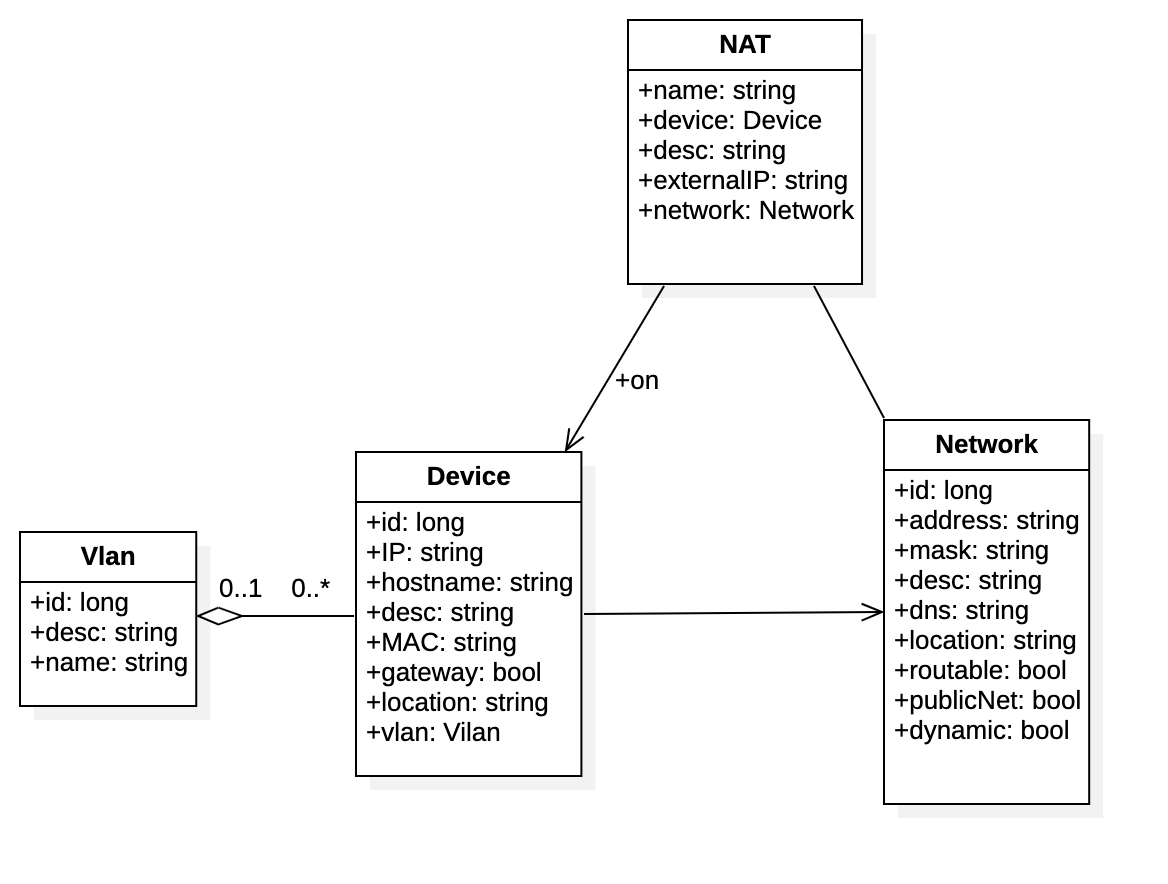
\includegraphics[width=8cm]{BuissnessClasses}
	\centering
\end{figure}

\subsection{Abstrakcyjny model interfejsu}
\begin{figure}[H]
	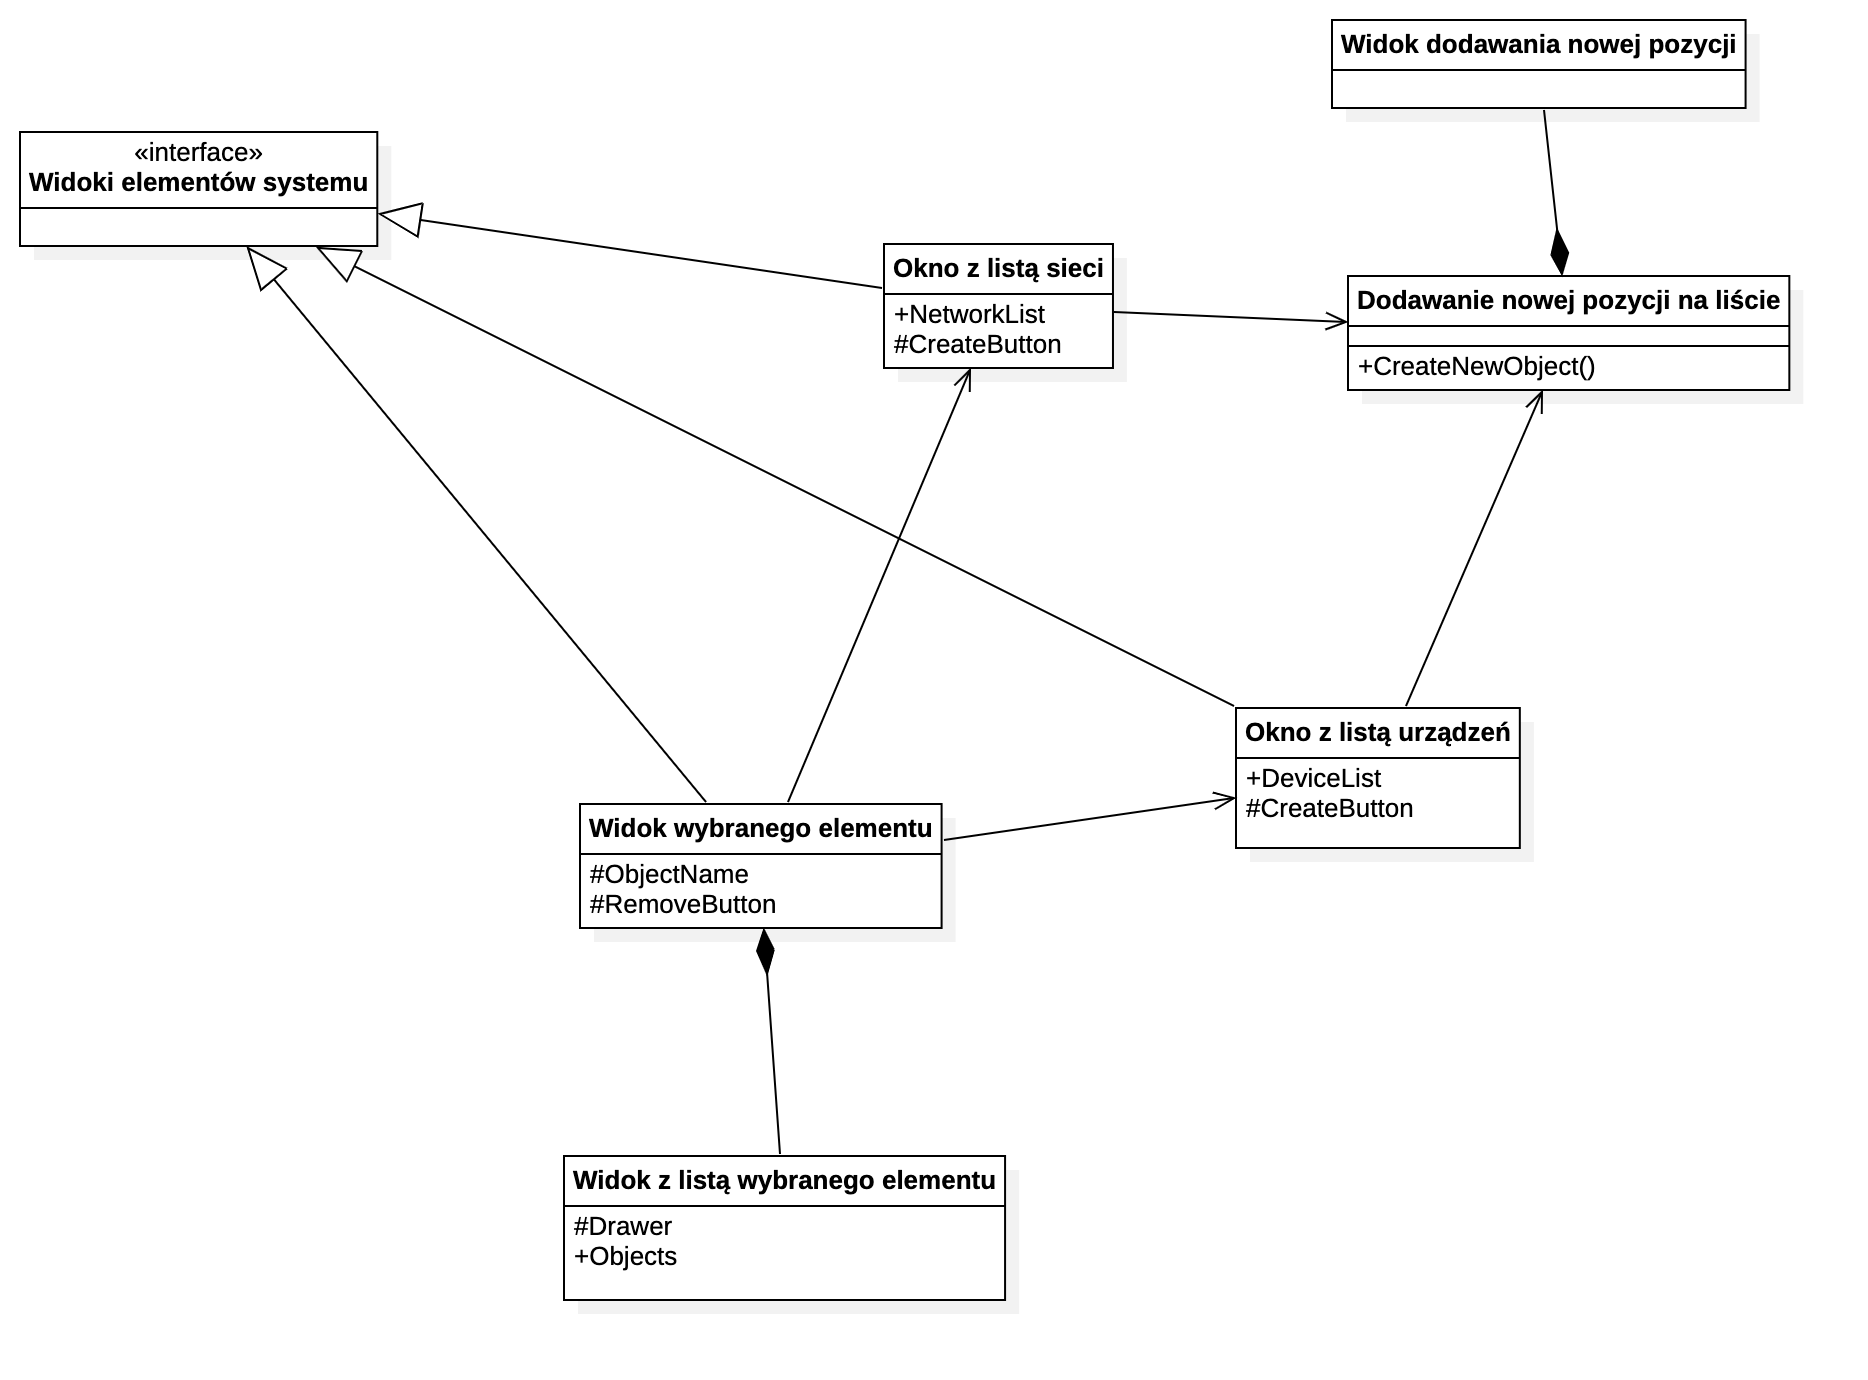
\includegraphics[width=8cm]{AbstractArchitectureDiagram}
	\centering
\end{figure}

\subsection{Diagram komponentów}
\begin{figure}[H]
	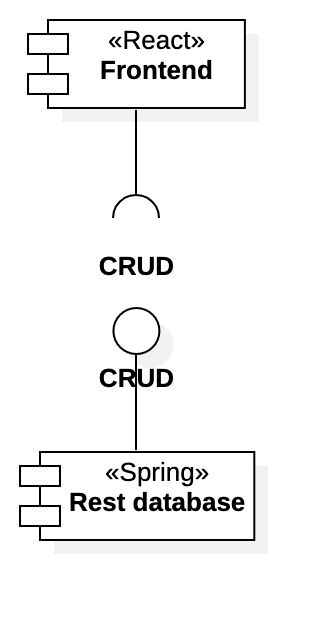
\includegraphics[height=8cm]{ComponentDiagram}
	\centering
\end{figure}

\subsection{Diagram sekwencji}
\begin{figure}[H]
	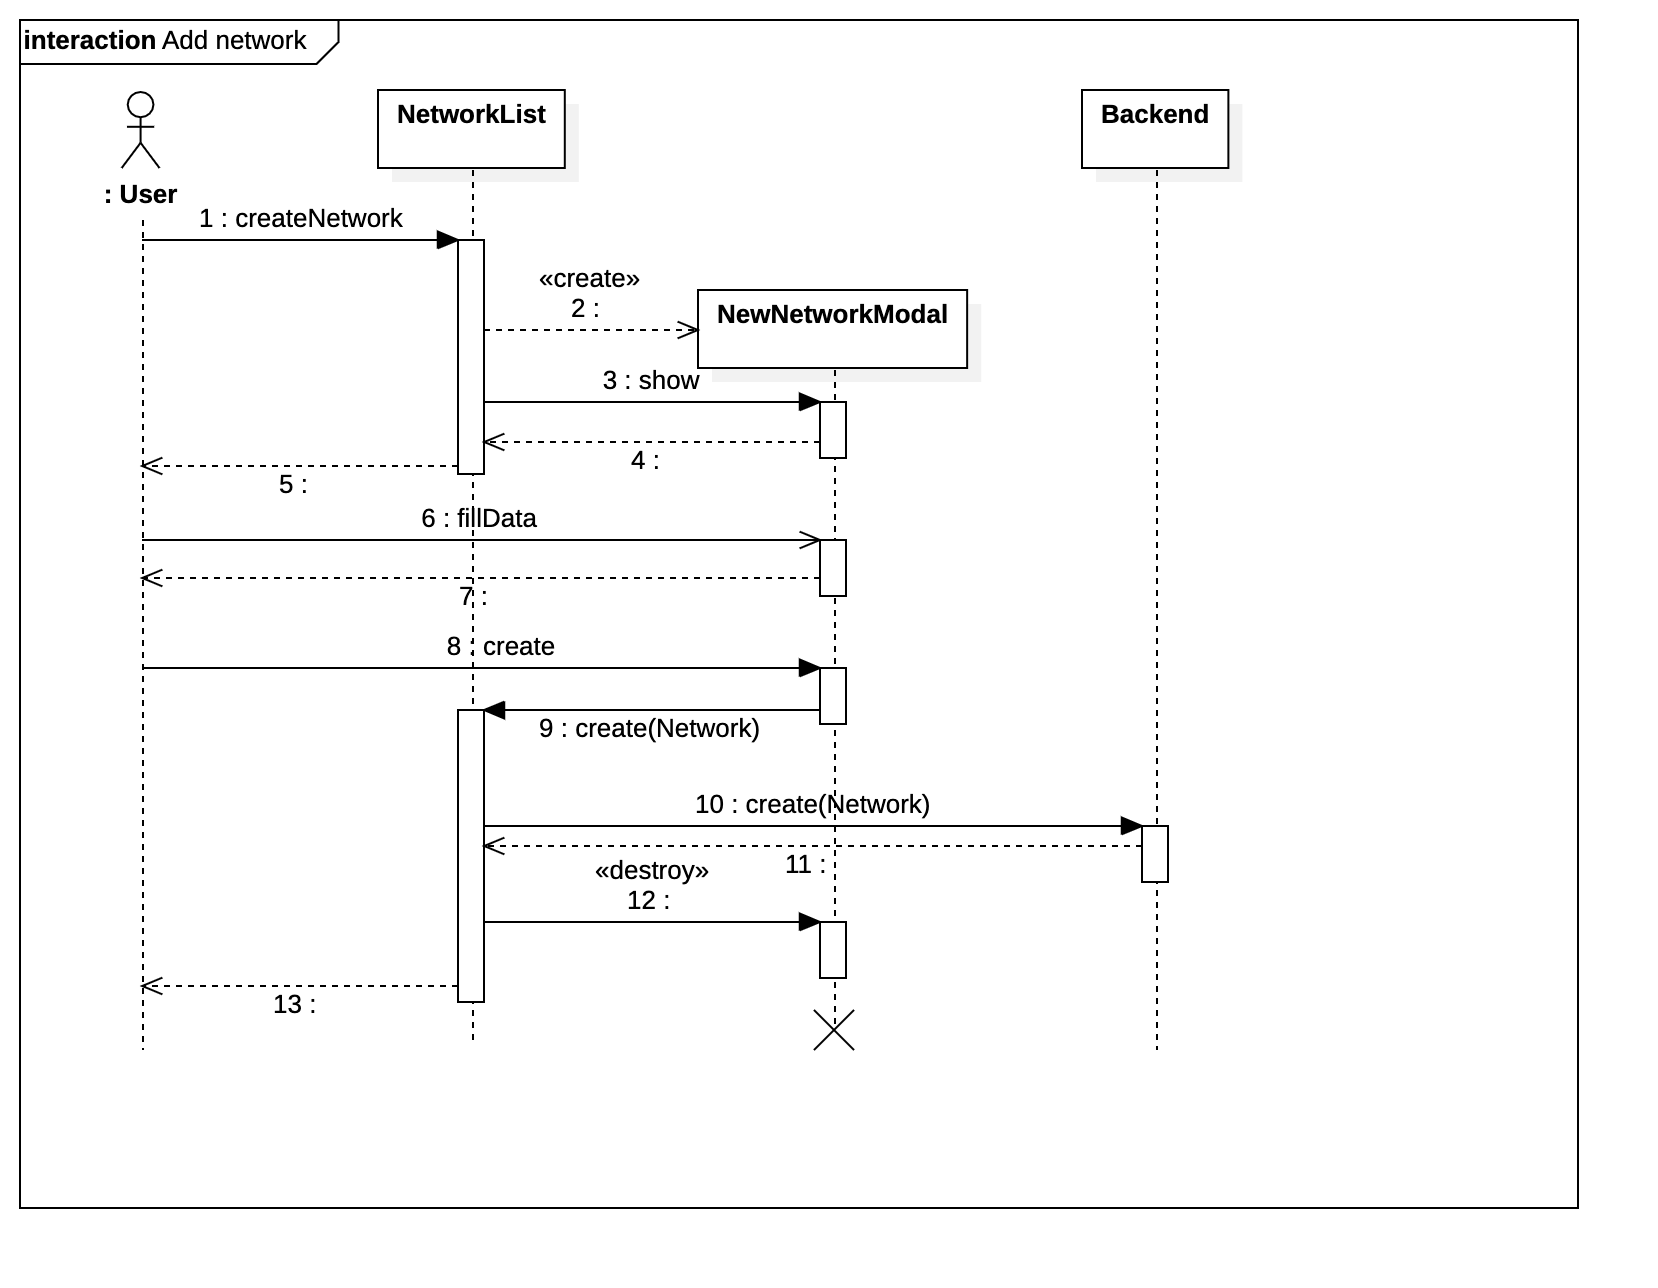
\includegraphics[width=8cm]{AddNetworkSequenceDiagram}
	\centering
\end{figure}

\subsection{Diagram stanów}
\begin{figure}[H]
	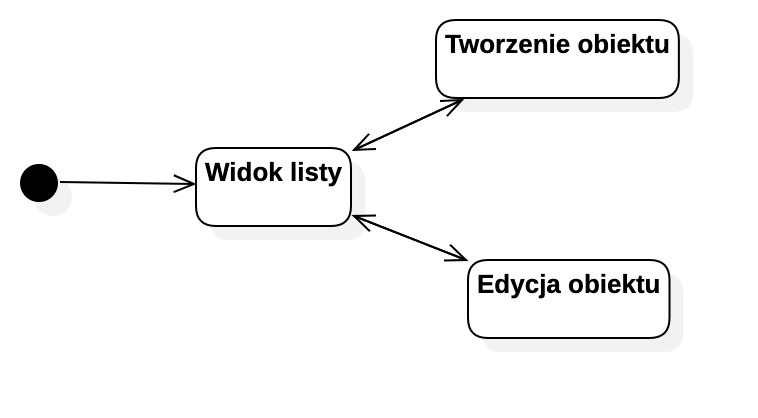
\includegraphics[width=8cm]{StateDiagram}
	\centering
\end{figure}

\section{Instrukcja zadaniowa}
\subsection{Dodanie nowej sieci}
Należy wejść na stronę związaną z sieciami i nacisnąć przycisk \texttt{CREATE}.
\begin{figure}[H]
	\centering
	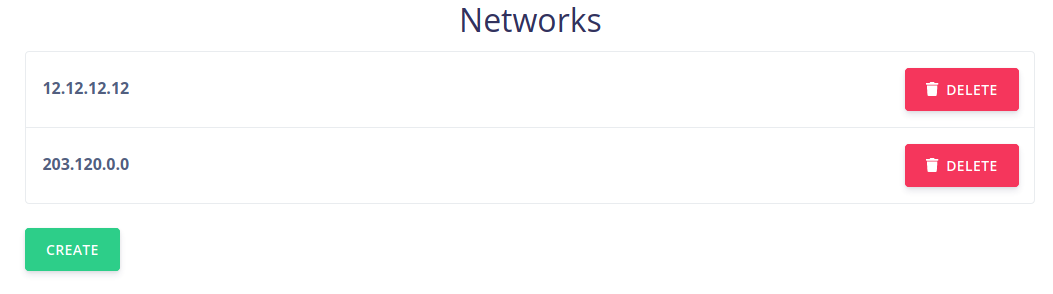
\includegraphics[width=10cm]{instr01.png}
\end{figure}
Następnie należy wypełnić formularz dodawania sieci.
\begin{figure}[H]
	\centering
	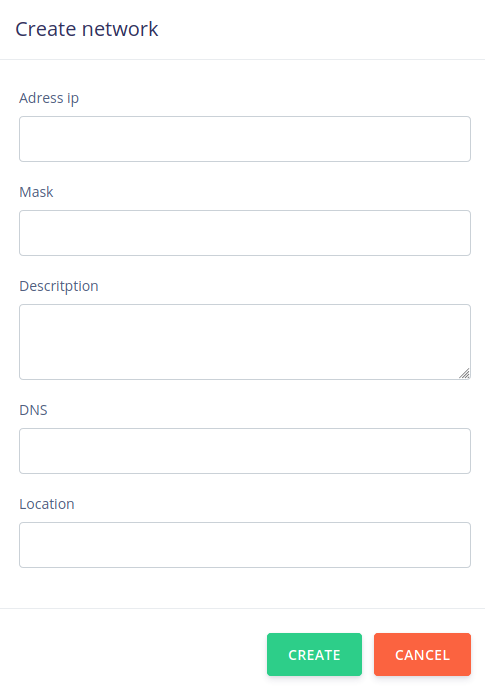
\includegraphics[width=10cm]{instr02.png}
\end{figure}
Po wypełnieniu informacji, nowa sieć pokaże się na liście.
\begin{figure}[H]
	\centering
	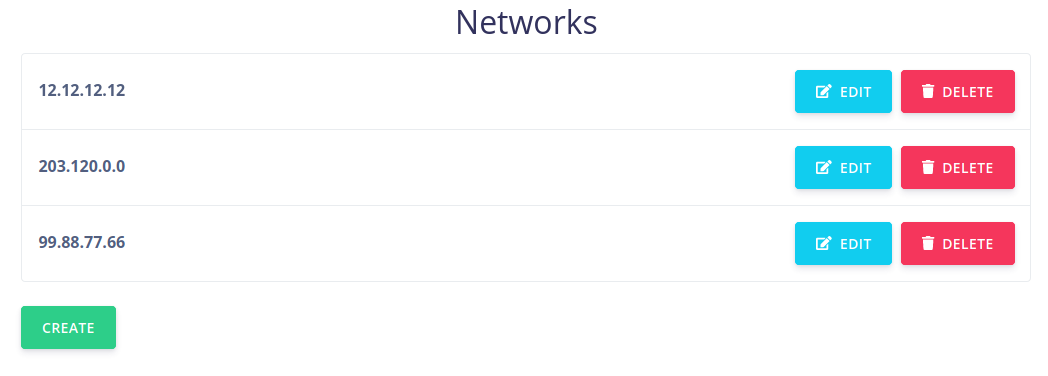
\includegraphics[width=10cm]{instr03.png}
\end{figure}

\subsection{Usuwanie sieci z listy}
Należy wejść na stronę związaną z sieciami i nacisnąć przycisk \texttt{DELETE} przy wybranej sieci.
\begin{figure}[H]
	\centering
	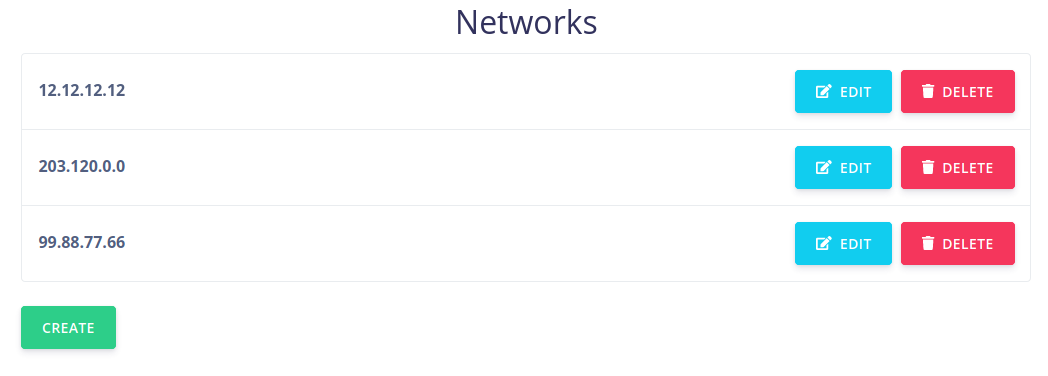
\includegraphics[width=10cm]{instr03.png}
	\caption{Przed usunięciem}
\end{figure}

\begin{figure}[H]
	\centering
	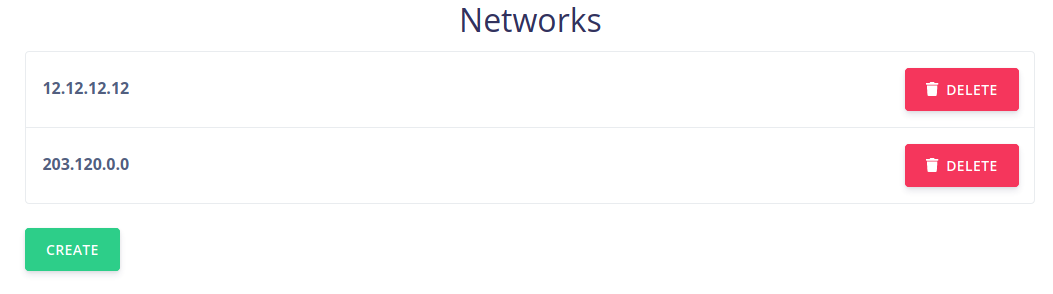
\includegraphics[width=10cm]{instr01.png}
	\caption{Po usunięciu}
\end{figure}


\end{document}